\subsection{Limiter les déchets, en facilitant le remplacement des pièces }

Dans la partie \ref{c1/s1/ss1:preuve_op}, nous citions l'exemple des iPods d'apple, dont la batterie était collée. Lorsque celle-ci tombait en panne,  l'appareil entier était à changer. 
Cet exemple est loin d'être un cas à part. N'importe quel ordinateur portable est soumis à cette obsolescence fonctionnelle. Lorsque la carte mère d'un PC arrête de fonctionner, il est quasiment impossible de réparer l'ordinateur. Pourtant, la pièce responsable de la panne est seulement un support sur laquelle sont implantés d'autres composants, qui restent fonctionnel après la mort de la carte mère.  

A l'inverse, dans le monde des ordinateurs fixes, une solution existe qui permet de contourner l'obsolescence fonctionnelle : monter soi-même son PC. Chaque pièce, choisie par l'utilisateur, est amovible. En cas de panne, prenons l'exemple de la carte graphique, il est facile de remplacer la pièce abîmée. Ainsi, l'\op peut être réduite de cette façon. 


Cette idée peut-elle être étendue ? 

\bigbreak

Des possibilités émergent dans le monde du smartphone. En 2013, Dave Hakkens propose de créer un téléphone modulable. Chaque pièce peut être changée au goût de l'utilisateur. Depuis la sortie de ce projet, de nombreux concurrents ont vu le jour : Google développe le projet Ara,  l'entreprise finlandaise \textit{Circular Devices OY} a dévoilé en décembre 2014 sa version de smartphone modulaire : le Puzzlephone. Les trois projets sont censés arriver sur le marché durant l'année 2015, cependant, aucune date officielle n'a encore été fixée. Il reste fort probable qu'un smartphone modulable sortira dans les prochaines années. 
\begin{figure}[h]
\begin{minipage}{0.5\linewidth}
\begin{center}
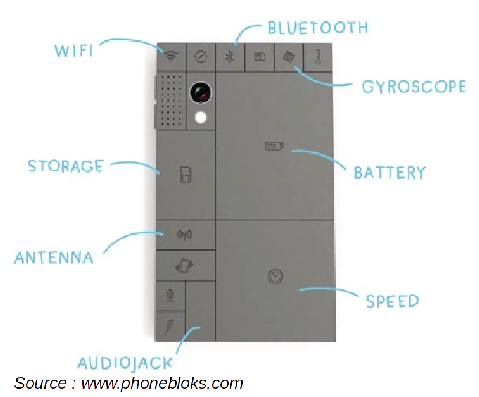
\includegraphics[scale=0.6]{Rsc/phonebloks2.png} 
\end{center}
\end{minipage}
\begin{minipage}{0.5\linewidth}
\begin{center}
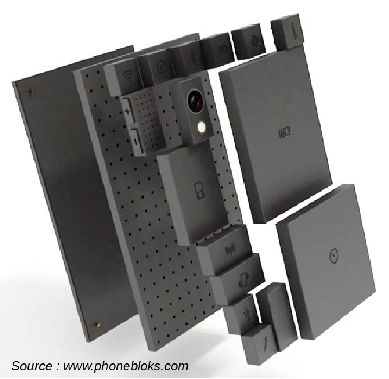
\includegraphics[scale=0.7]{Rsc/phonebloks1.png} 
\end{center}
\end{minipage}
\caption{\scriptsize{Phonebloks : le téléphone qui se monte et se démonte en quelques secondes.}}
\label{phonebloks}
\end{figure}

Cependant, de nombreuses critiques sont faites par rapport à ces projets. Ils sont à la base portés sur le Phonebloks, qui est l'élément fondateur. D'après  Bruno Salgues \cite{phonebloks_critiques} , directeur des études à l'Institut Mines-Télécom, le téléphone est réalisable. Malgré cela, il soulève un point  dérangeant pour l'image écologique des téléphones modulables : la compatibilité entre la base du téléphone et les différents blocs qu'on vient greffer dessus pourrait être polluante. Il explique : \og{}\textit{Dans un smartphone, il existe les logiciels gravés dans la puce de l’appareil et ceux qui sont dans sa mémoire, rappelle Bruno Salgues. Avec Phonebloks, comment faire en sorte que les logiciels permettant d'activer les différents composants soient compatibles avec la puce du téléphone [en cas de renouvellement de la base] ?}\fg{}. 

\medbreak 

L'émergence de téléphones modulables dans quelques années est donc probable, même s'il n'est pas sûr que cette méthode soit plus écologique que dans le cas de téléphone non modulable. 

L'idée plus récente de Dave Hakkens est d'étendre son concept à d'autres objets. Dans sa deuxième vidéo\footnote{\href{https://www.youtube.com/watch?v=4KmewIC-eV4}{Youtube : \textit{Phonebloks - Our first year}}}, le développeur propose d'étendre son idée aux télévisions ou aux laves-linges. Il créerait ainsi une machine à laver modulable. Même si l'idée est intéressante, le problème identique, cité par Bruno Salgues subsiste. Attendons donc les résultats du Phonebloks avant de s'intéresser aux lave-linges. 

\bigbreak

Remplacer une partie d'un produit est une pratique très courante dans le cas des voitures. 
Ainsi, un garagiste consciencieux ne va pas déclarer que la voiture est hors d'usage lors de la rupture d'une courroie, mais proposera de remplacer la pièce défectueuse. Il a alors deux possibilités : acheter une nouvelle courroie, ou en trouver une d'occasion. Dans ce cas, on parle d'économie circulaire : on réinjecte des parties de produits hors d'usage dans le marché. C'est un rôle important des casses automobiles, qui permettent de racheter des pièces que les employés auront extraites des restes de voitures. 

La réparation est un domaine bien plus vaste que les automobiles. Intéressons-nous maintenant au différentes possibilités de dépannage de produits considérés comme hors-service. 